\documentclass[a4paper]{article}
\usepackage[utf8]{inputenc}
\usepackage[spanish, es-tabla, es-noshorthands]{babel}
\usepackage[table,xcdraw]{xcolor}
\usepackage[a4paper, footnotesep = 1cm, width=18cm, left=2cm, top=2.5cm, height=25cm, textwidth=18cm, textheight=25cm]{geometry}
%\geometry{showframe}

\usepackage{amsmath}
\usepackage{amsfonts}
\usepackage{amssymb}
\usepackage{float}
\usepackage{graphicx}
\usepackage{caption}
\usepackage{subcaption}
\usepackage{multicol}
\usepackage{multirow}
\setlength{\doublerulesep}{\arrayrulewidth}

\graphicspath{{../Ejercicio-1/}{../Ejercicio-2/}{../Ejercicio-3y4/}{../Ejercicio-5-6y7/}{../Ejercicio-8/}}

\usepackage{hyperref}
\hypersetup{
    colorlinks=true,
    linkcolor=blue,
    filecolor=magenta,      
    urlcolor=blue,
    citecolor=blue,    
}
\newcommand\underrel[2]{\mathrel{\mathop{#2}\limits_{#1}}}
\newcommand{\quotes}[1]{``#1''}
\usepackage{array}
\newcolumntype{C}[1]{>{\centering\let\newline\\\arraybackslash\hspace{0pt}}m{#1}}
\usepackage[american,oldvoltagedirection,siunitx]{circuitikz}
\usepackage{fancyhdr}
\usepackage{units}
\usepackage{booktabs}

\usepackage{tikz}
\usetikzlibrary{babel}

\pagestyle{fancy}
\fancyhf{}
\lhead{22.42 Laboratorio de Electrónica}
\rhead{Bertachini, Lambertucci, Londero Bonaparte, Mechoulam, Scapolla}
\rfoot{\center \thepage}

\begin{document}

Para la siguiente sección, se buscó diseñar un puente que permita medir capacitores desde $100 \ nF$ hasta $1 \ \mu F$, trabajando a una frecuencia de $20 \ kHz$. Los capacitores a medir con dicho instrumento se caracterizan por poseer un factor de disipación D en un rango acotado entre $0.02$ y $0.12$.

Con lo dicho anteriormente, se tuvo que elegir entre tres posibles puentes: el serie, el paralelo y el de Schearing. Debido a que este último se emplea para capacitores con de muy bajas perdidas, es decir, con un $D \ < \ 10^{-3}$, mientras que el paralelo se utiliza para capacitores de altas perdidas, se optó por valerse de un puente serie, ya que este está destinado a ser empleado en un rango de perdidas similar al que requiere.

\begin{figure}[H]
\begin{center}
\begin{circuitikz}[european voltages]
%	\draw (0,0) to[rmeterwa, t=V, label=$V_d$] ++(3,0) to[R, l=$R_4$] ++(0,-2) to[short] ++(-4,0) node[ocirc](-vg){};
\draw (0,0) to[short] ++(3,0) to[R, l=$R_4$] ++(0,-2) to[short] ++(-4,0) node[ocirc](-vg){};
	\draw (0,0) to[vR, mirror, l=$R_3$] ++(0,-2);
	\draw (0,1.5) to[vR, mirror, l=$R_1$] (0,0);
	\draw (0,1.5) to[C, l_=$C_1$] ++(0,1.5) to[short] ++(3,0) to[C, l=$C_x$] ++(0,-1.5) to[R, l =$R_x$] ++(0,-1.5);
	\draw (0,3) to[short] ++(-1,0) node[ocirc](vg){};
	\draw (-vg) to[open, v^= $V_g$] (vg);
\end{circuitikz}
	\caption{Puente serie implementado}
	\label{fig:puenteserie}
\end{center}
\end{figure}

Luego, mediante el análisis de sensibilidades, considerando los valores máximos y mínimos de capacitores y estableciendo $C_1 = 1 \ nF$ y $R_1 = 100 \ \Omega$, se obtienen los siguientes valores para los demás componentes:

\begin{equation*}
\begin{split}
	R_{1_{Min}} =& \ \frac{5 \cdot 10^{-7}}{\pi C_1} = 159 \ \Omega \\
	R_{1_{Max}} =& \ \frac{3 \cdot 10^{-6}}{\pi C_1} = 1 \ k\Omega \\
	R_{3_{Min}} =& \ \frac{R_4 \cdot 10^{-7}}{\pi C_1} = 10 \ k\Omega \\
	R_{3_{Max}} =& \ \frac{R_4 \cdot 10^{-6}}{\pi C_1} = 100 \ k\Omega
\end{split}
\end{equation*}

Se realizó el análisis de sensibilidades para la tensión $Vd$, observando su variación en funcion de $R_1$ y $R_3$:
\begin{align*}
\scalebox{1.5}{$
S_{R_1}^{V_d} = \frac{\partial V_d}{\partial R_1} \cdot \frac{R_1}{V_d}=
\frac{-R_1R_3}{\left( \frac{R_3}{R_3+\frac{1}{sC_1}+R1}-\frac{R_4}{R_4+\frac{1}{sC_x}+R_x} \right) \cdot  \left( R_3+\frac{1}{sC_1}+R1\right)^2}
$}
\end{align*}

\begin{align*}
\scalebox{1.5}{$
S_{R_3}^{V_d} = \frac{\partial V_d}{\partial R_3} \cdot \frac{R_3}{V_d}=\frac{(C_1R_1s+1)R_3C_1(C_xR_xs+R_4C_xs+1)}{(C_1R_1s+C_1R_3s+1)\cdot (-C_1C_xR_3R_xs+R_4C_1C_xR_1s-C_1R_3+R_4C_x)}
$}
\end{align*}

Luego, fijando la frecuencia, se graficó la tensión del puente en función de las resistencias previamente mencionadas.
\begin{figure}[H]
	\centering
	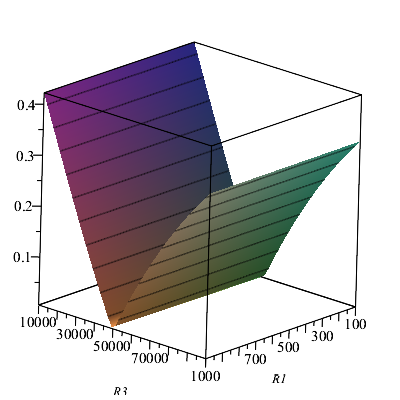
\includegraphics[width=0.4\textwidth]{/ImagenesEjercicio3/Graph.png}
	\label{fig:graph}
\end{figure}

También se realizó una simulación de Montecarlo para asegurar que el puente converja al equilibrio.
\begin{figure}[H]
	\centering
	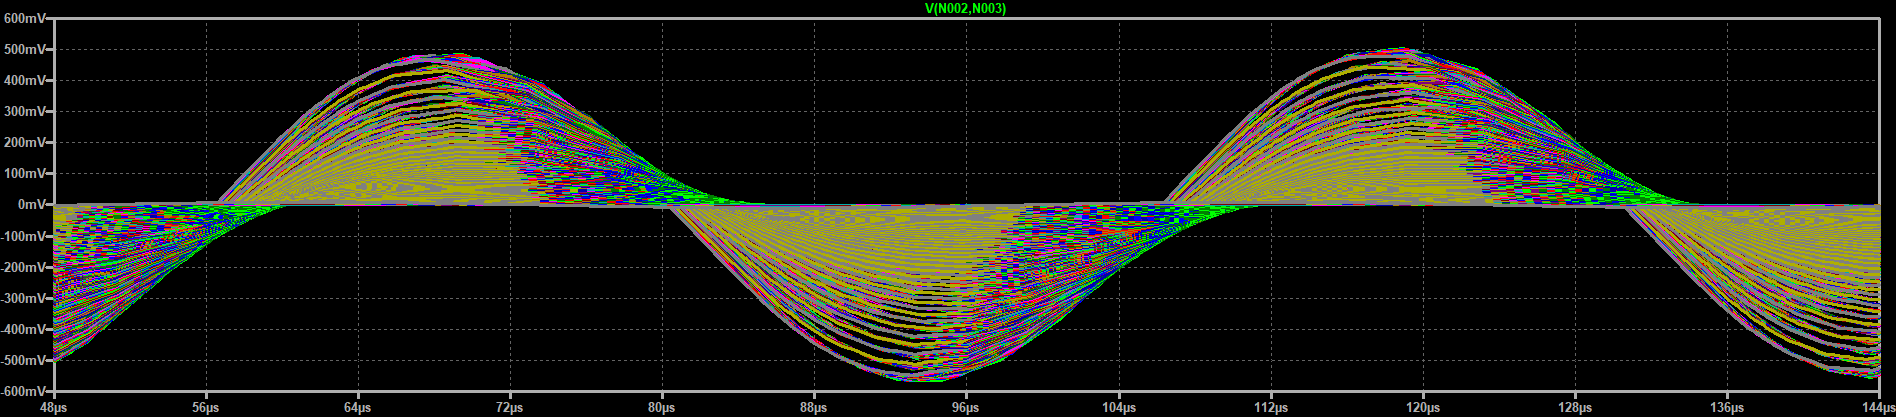
\includegraphics[width=\textwidth]{/ImagenesEjercicio3/Montecarlos.png}
	\label{fig:graph}
\end{figure}

Planteando la tensión en el equilibrio, y despejando algebraicamente, se llega a las siguientes expresiones:
\begin{equation*}
\begin{split}
	C_{x} =& \ \frac{C_1R_3}{R_4}\ F \\
	R_{x} =& \ \frac{R_1R_4}{R_3}\ \Omega \\
	D_{x} =& \ 2\pi f C_1R_1 
\end{split}
\end{equation*}

A partir de estas, se puede calcular la precisión del puente para estos parámetros:
\begin{equation*}
\begin{split}
	\Delta C_{x} =& \ \frac{C_1 \cdot \Delta R_3}{R_4}\  \\
	\Delta R_{x} =& \ \frac{\Delta R_1 \cdot R_4  R_3+R_1  R_4 \cdot \Delta R_3}{(R_3)^2}\  \\
	\Delta D_{x} =& \ 2\pi f C_1 \Delta R_1 
\end{split}
\end{equation*}

Obteniendo para cada capacitor una medición del punto de estabilización del puente.

% Please add the following required packages to your document preamble:
% \usepackage{multirow}
\begin{table}[H]
\scalebox{0.65}{
\centering
\begin{tabular}{|c|c|c|c|c|c|c|c|c|c|c|c|c|c|c|c|c|c|c|c|}
\hline
\multirow{2}{*}{\textit{Valor nominal}} & \multicolumn{6}{c|}{2Khz}                       & \multicolumn{6}{c|}{20KHz}                      & \multicolumn{6}{c|}{200KHz}                  & \multirow{2}{*}{Observaciones}                                                                                                                 \\ \cline{2-19}
                                        & C       & D     & $\phi$ & C       & D & $\phi$ & C       & D     & $\phi$ & C       & D & $\phi$ & C      & D     & $\phi$ & C     & D & $\phi$ &                                                                                                                                                \\ \hline
100 nF                                   & 99.83 nF & 0.012 & 0      & 102 nF   & x & -4     & 114.1 nF & 0.022 & 0      & 101 nF   & x & 1      & 98.9 nF & 0.125 & 4      & 120 nF & x & 4      & -                                                                                                                                              \\ \hline
500 nF                                   & 507 nF   & x     & -1     & 494.6 nF & 4 & x      & 507 nF   & x     & 1      & 514.6 nF & x & 6      & 530 nF  & x     & 1      & 540 nF & 1 & 4      & -                                                                                                                                              \\ \hline
1 $\mu$F                                     & 1 $\mu$F     & x     & 0      & 1 $\mu$F     & x & 6      & 1 $\mu$F     & x     & 0      & 1 $\mu$F     & x & 1      & 1 $\mu$F    & x     & 0      & 1 $\mu$F   & x & 0      & -                                                                                                                                              \\ \hline
2 $\mu$F                                     & 1 $\mu$F     & x     & 24     & 1 $\mu$F     & x & 25     & 1 $\mu$F     & x     & 4      & 1 $\mu$F     & x & 4      & 1 $\mu$F    & x     & 1      & 1 $\mu$F   & x & 1      & \begin{tabular}[c]{@{}c@{}}El puente no llega al equilibrio\\  dado que se encuentra fuera del rango \\ para el cual fue diseñado\end{tabular} \\ \hline
\end{tabular}
}
\end{table}
%%%%%%%%%%%%100 NANO
\begin{figure}[H]
	\centering
	\includegraphics[width=0.4\textwidth,trim={0 2.2cm 0.1cm 1.75cm},clip]{/Mediciones/minimo/1xxnD0.x/2kHz.png}
	\includegraphics[width=0.4\textwidth,trim={0 2.2cm 0.1cm 1.75cm},clip]{/Mediciones/minimo/100nD0.02/2kHz.png}
	\subcaption{Medición de 100 nF a 2 kHz con distinto D [Derecha 0.012].}
	\label{fig:fcon}
\end{figure}
\begin{figure}[H]
	\centering
	\includegraphics[width=0.4\textwidth,trim={0 2.2cm 0.1cm 1.75cm},clip]{/Mediciones/minimo/1xxnD0.x/20kHz.png}
	\includegraphics[width=0.4\textwidth,trim={0 2.2cm 0.1cm 1.75cm},clip]{/Mediciones/minimo/100nD0.02/20kHz.png}
\caption{Medición de 100 nF a 20 kHz con distinto D [Derecha 0.012].}
	\label{fig:fcon}
\end{figure}
\begin{figure}[H]
	\centering
	\includegraphics[width=0.4\textwidth,trim={0 2.2cm 0.1cm 1.75cm},clip]{/Mediciones/minimo/1xxnD0.x/200kHz.png}
	\includegraphics[width=0.4\textwidth,trim={0 2.2cm 0.1cm 1.75cm},clip]{/Mediciones/minimo/100nD0.02/200kHz.png}
\caption{Medición de 100 nF a 200 kHz con distinto D [Derecha 0.012].}
	\label{fig:fcon}
\end{figure}
%%%%%%%%%%%%500 nano
\begin{figure}[H]
	\centering
	\includegraphics[width=0.4\textwidth,trim={0 2.2cm 0.1cm 1.75cm},clip]{/Mediciones/media/4xxD0.x/2kHz.png}
	\includegraphics[width=0.4\textwidth,trim={0 2.2cm 0.1cm 1.75cm},clip]{/Mediciones/media/406nD0.02/2kHz.png}
\caption{Medición de 500 nF a 2 kHz con distinto D [Derecha 0.012].}
	\label{fig:fcon}
\end{figure}
\begin{figure}[H]
	\centering
	\includegraphics[width=0.4\textwidth,trim={0 2.2cm 0.1cm 1.75cm},clip]{/Mediciones/media/4xxD0.x/20kHz.png}
	\includegraphics[width=0.4\textwidth,trim={0 2.2cm 0.1cm 1.75cm},clip]{/Mediciones/media/406nD0.02/20kHz.png}
\caption{Medición de 500 nF a 20 kHz con distinto D [Derecha 0.012].}
	\label{fig:fcon}
\end{figure}
\begin{figure}[H]
	\centering
	\includegraphics[width=0.4\textwidth,trim={0 2.2cm 0.1cm 1.75cm},clip]{/Mediciones/media/4xxD0.x/200kHz.png}
	\includegraphics[width=0.4\textwidth,trim={0 2.2cm 0.1cm 1.75cm},clip]{/Mediciones/media/406nD0.02/200kHz.png}
\caption{Medición de 500 nF a 200 kHz con distinto D [Derecha 0.012].}
	\label{fig:fcon}
\end{figure}
%%%%%%%%%%%%1 micro
\begin{figure}[H]
	\centering
	\includegraphics[width=0.4\textwidth,trim={0 2.2cm 0.1cm 1.75cm},clip]{/Mediciones/maximo/1xud0.x/2kHz.png}
	\includegraphics[width=0.4\textwidth,trim={0 2.2cm 0.1cm 1.75cm},clip]{/Mediciones/maximo/1ud0.2/2kHz.png}
\caption{Medición de 1 $\mu$F a 2 kHz con distinto D [Derecha 0.012].}
	\label{fig:fcon}
\end{figure}
\begin{figure}[H]
	\centering
	\includegraphics[width=0.4\textwidth,trim={0 2.2cm 0.1cm 1.75cm},clip]{/Mediciones/maximo/1xud0.x/20kHz.png}
	\includegraphics[width=0.4\textwidth,trim={0 2.2cm 0.1cm 1.75cm},clip]{/Mediciones/maximo/1ud0.2/20kHz.png}
\caption{Medición de 1 $\mu$F a 20 kHz con distinto D [Derecha 0.012].}
	\label{fig:fcon}
\end{figure}
\begin{figure}[H]
	\centering
	\includegraphics[width=0.4\textwidth,trim={0 2.2cm 0.1cm 1.75cm},clip]{/Mediciones/maximo/1xud0.x/200kHz.png}
	\includegraphics[width=0.4\textwidth,trim={0 2.2cm 0.1cm 1.75cm},clip]{/Mediciones/maximo/1ud0.2/200kHz.png}
\caption{Medición de 1 $\mu$F a 200 kHz con distinto D [Derecha 0.012].}
	\label{fig:fcon}
\end{figure}
%%%%%%%%%%%%%2 micro
\begin{figure}[H]
	\centering
	\includegraphics[width=0.4\textwidth,trim={0 2.2cm 0.1cm 1.75cm},clip]{/Mediciones/doblemaximo/2xud0.x/2kHz.png}
	\includegraphics[width=0.4\textwidth,trim={0 2.2cm 0.1cm 1.75cm},clip]{/Mediciones/doblemaximo/2ud0.2/2kHz.png}
\caption{Medición de 2 $\mu$F a 2 kHz con distinto D [Derecha 0.012].}
	\label{fig:fcon}
\end{figure}
\begin{figure}[H]
	\centering
	\includegraphics[width=0.4\textwidth,trim={0 2.2cm 0.1cm 1.75cm},clip]{/Mediciones/doblemaximo/2xud0.x/20kHz.png}
	\includegraphics[width=0.4\textwidth,trim={0 2.2cm 0.1cm 1.75cm},clip]{/Mediciones/doblemaximo/2ud0.2/20kHz.png}
\caption{Medición de 2 $\mu$F a 20 kHz con distinto D [Derecha 0.012].}
	\label{fig:fcon}
\end{figure}
\begin{figure}[H]
	\centering
	\includegraphics[width=0.4\textwidth,trim={0 2.2cm 0.1cm 1.75cm},clip]{/Mediciones/doblemaximo/2xud0.x/200kHz.png}
	\includegraphics[width=0.4\textwidth,trim={0 2.2cm 0.1cm 1.75cm},clip]{/Mediciones/doblemaximo/2ud0.2/200kHz.png}
\caption{Medición de 2 $\mu$F a 200 kHz con distinto D [Derecha 0.012].}
	\label{fig:fcon}
\end{figure}

Finalmente se realizaron las mismas mediciones en el analizador de impedancias para obtener un calculo del error, obteniendo las siguientes mediciones.\\
\begin{center} 
	\begin{Huge}
		\textcolor{red}{\textbf{TABLA ANALIZADOR DE IMPEDANCIAS.}}
	\end{Huge}
\end{center}

Luego el error fue calculado utilizando la siguiente fórmula:
\begin{equation*}
\begin{split}
	 Error \% =& \ \frac{|C_{Gen}-C_{Puente}|}{C_{Puente}}\ 
\end{split}
\end{equation*}
\end{document}